\documentclass[a4paper]{article}
\usepackage{chemfig}
\usepackage{mhchem}
\usepackage{xcolor}
\usepackage{amsmath}
\usepackage{tikz}
\begin{document}
\section{Thermodynamik für Knechte}
\subsection{Was ist Thermodynamik?}
Thermodynamik:
\begin{itemize}
    \item makroskopische Skala
    \item Umwandlungen von Energie
    \begin{itemize}
        \item Austausch von Wärme
        \item Leistung von Arbeit
    \end{itemize}
    \item Gleichgewicht
    \item Richtung von spontanen Prozessen
\end{itemize}
Chemische Thermodynamik: Lage der chemischen Gleichgewichte\\
\hspace*{1cm} Wärmeeffekte dhemischer Reaktionen\\
Technische Thermodynamik: Umsetzung von Wärme und Arbeit\\
\begin{equation*}
    \ce{N2 + 3H2 -> 2NH3}    
\end{equation*}
\begin{center}
    250$-$300 bar\\
    450$-$550°
\end{center}
\ce{MeOH} Automobilantrieb:\\
\ce{CH3OH + \frac{3}{2}O2 -> CO2 + H2O}\\
\\
Anode\\
\hspace*{1cm} \ce{CH3OH + H2O -> 6H+ + 6e- + CO2}\\
Kathode\\
\hspace*{1cm} \ce{\frac{3}{2}O2 + 6H+ + 6e- -> 3H2O}\\
\subsection{Thermodynamische Systeme}
Definitionen:\\
\underline{System:} \hspace*{1.55cm} Der Teil des Universums, der uns interessiert\\
\underline{Umgebung:} \hspace*{1cm} Der Rest \hspace*{0.5cm} (der im Kontakt mit dem System steht)\\
\\
Grenze ist die \underline{Systemgrenze} \hspace*{0.5cm} (Wand)
\begin{center}
    \begin{tabular}{c c c} 
     \hline
     System & Materienaustausch & Energieaustausch \\ 
     \hline
     isoliert & $-$ & $-$ \\ 
     geschlossem & $-$ & $+$ \\ 
     offen & $+$ & $+$\\
     \hline
    \end{tabular}
    \end{center}
\subsubsection{Phase}
Bereich ohne Sprunghafte Änderung
\begin{itemize}
    \item chemische Zusammensetzung
    \item physikalische Eigenschaften
    \item Aggregatzustände
\end{itemize}
Komponenten
\begin{itemize}
    \item chemisch unterscheidbare Bestandteile (Stoffe)
\end{itemize}
Modifikationen von Elementen: Allotrope
\subsubsection{Aggregatzustände}
\begin{itemize}
    \item Teilchenabstand
    \item Teilchenordnung
\end{itemize}
$R$ ist der Abstand zwischen den Zentren zweier Atome, und $d$ ist der Durchmessser eines Atomes.\\
Gasförmig:\\
$R >> d$\\
keine Ordnung\\
\\
Flüssig:\\
$R \approx d$\\
Nahordnung\\
\\
Fest:\\
$R \approx d$\\
Fernordnung = Kristallin\\
Nahordnung = Amorph\\
\\
Es gibt noch Plasma, dabei haben sich Elektronen und Atomkerne separiert\\
\subsubsection{Gleichgewicht}
Mechanisch:
\begin{equation*}
    \sum \vec{F} = 0, \sum \vec{\tau} = 0
\end{equation*}
Anmerkung $\tau$ ist hier das Drehmoment\\\\
Thermisch:
\begin{equation*}
    \Delta T = T_{ex} - T_{in} = 0
\end{equation*}
\\
Chemisch:\\
Chemische Potentiale \textcolor{gray}{(von Edukten/Produkten)} sind gleich.\\
\begin{center}
    Dynmaisches Gleichgewicht $\leftrightarrow$ Fließgleichgewicht
\end{center}
\subsubsection{0. Hauptsatz der Thermodynamik}
\begin{equation*}
    T_a \neq T_b \neq T_c -\Delta E -> T_a = T_b = T_c
\end{equation*}
$T_a = T_b$\\
a,b im thermischen Gleichgewicht\\\\
und $T_b = T_c$\\
b,c im thermischen GLeichgewicht\\\\
dann muss auch $T_a = T_b$ gelten\\
a,c im thermischen Gleichgewicht.\\\\
TD: thermodynamische oder absolute Temperatur $T$[K]\\
Celsiustemperatur $\vartheta$[°C]\\
$\vartheta$ = $T$ - 273,15
\subsection{Zustandsgrößen}
\underline{Zustand:}\\
\hspace*{1cm}Beschaffenheit des Systems\\
\hspace*{1.5cm}$\rightarrow$Alle Infos um das System eindeutig beschreiben zu können\\\\
\underline{Zustandsgrößen:}\\
\hspace*{1cm} $T, V, p, H$ \textcolor{gray}{(Enthalpie)} $, S$ \textcolor{gray}{(Entropie)}\\
\hspace*{1cm} Änderungen sind wegunabhängig: $\left|\Delta A \right|$\\\\
\underline{Prozessgrößen:}\\
\hspace*{1cm} $q$ \textcolor{gray}{(Wärme)}, $W$ \textcolor{gray}{(Arbeit)}, $F$ \textcolor{gray}{(Kraft)} beschreiben Zustandsänderungen\\
\subsubsection{intensive Zustandsgrößen \textcolor{gray}{(unabhängig von der Stoffmenge $n$ - \underline{in}dependent)}}
Temperatur $T$\\
Druck $p$\\
Dichte $\rho$\\
Viskosität $\eta$\\
\subsubsection{extensive Zustandsgrößen \textcolor{gray}{(abhängig von der Stoffmenge $n$)}}
Volumen $V$\\
Stoffmenge $n$\\
Innere Energie $U$\\
Entropie $S$\\
\subsubsection{Definition einer spezifische Größe \textcolor{gray}{(teilen durch Masse)}}
spezifisches Volumen $v$ = $\frac{V}{m}$
\subsubsection{Definition einer molaren Größe \textcolor{gray}{(teilen durch Stoffmenge)}}
molares Volumen $V_m$ = $\frac{V}{n}$
\subsubsection{verschiedene Größen}
Molmasse $M$ [$\frac{\mathrm{g}}{\mathrm{mol}}$]\\
1 Mol Tielchen = $6, 02 \cdot 10^{23}$ Teilchen\\
$N_A = 6.02 \cdot 10^{23} \frac{1}{\mathrm{mol}}$\\\\
Stoffmenge $n$ [mol] $=\frac{N}{N_\eta}=\frac{\mathrm{Masse}}{\mathrm{Molmasse}}=\frac{m}{M}$\\\\
Konzentration $c$ [$\frac{\mathrm{mol}}{\mathrm{l}}$] $= \frac{n}{V}$\\\\
Dichte $\rho$ [$\frac{\mathrm{kg}}{\mathrm{m}^3}$]\\\\
Molalität $b$ [$\frac{\mathrm{mol}}{\mathrm{kg}}$] $=\frac{\mathrm{Stoffmenge}}{\mathrm{Masse_{L\text{ö}M}}}=\frac{n}{m_{LM}}$\\\\
Partielle Größen\\
Molenbruch\\
\begin{equation*}
    x_i=\frac{n_i}{\sum_i n_i}
\end{equation*}
\subsubsection{thermodynamische Prozesse}
\begin{itemize}
    \item Volumenänderung ("Arbeit") $w = -p \Delta V$
    \item Temperatruänderung ("Wärmeaustausch") $q = c \delta T$ hierbei: $c =$ Wärmekapazität
    \item Phasenübergänge $q = \Delta H$
    \item chemische Reaktionen \ce{2A + B -> c}\\ \begin{equation*}
        n_c(t)=n_c(0)+\nu_i\xi
    \end{equation*}\\hierbei $\nu =$ Stöchiometrischer Koeffizient und $\xi =$ Reaktionsfortschritt
\end{itemize}
\begin{center}
    Prozessführung
    \begin{tabular}{c c c} 
        \hline
        Bezeichnung & Konstante Größe & Fachbegriff und Beschreinbung \\ 
        \hline
        Isotherm & $T$ & adiabatisch: ohne Wärmeaustausch \\ 
        Isobar & $p$ & reversibel: im ständigen Gleichgewicht\\ 
        Isochor & $V$ & irreversibel: nicht im Gleichgewicht\\
        \hline
       \end{tabular}
\end{center}
\subsection{Zustandsgleichung - Zusammenhang zwischen Zustandsgrößen}
\begin{equation*}
    A = B^2 + 3C
\end{equation*}
A ist hierbei die Zustandsgröße, B und C sin Zustandsvariablen.\\
Beispiel:
\begin{equation*}
    p = \frac{nRT}{V}
\end{equation*}
\\
\textbf{Totales Differential:}\\
\begin{equation*}
    Z = f(x,y)
\end{equation*}
\begin{equation*}
    dz=\left(\frac{\partial z}{\partial x}\right)_ydx+\left(\frac{\partial z}{\partial y}\right)_xdy
\end{equation*}
\section{Gase}
\subsection{Das ideale Gas}
\begin{tikzpicture}
    \draw (0,0) -- (7,0) -- (7,4) -- (0,4) -- (0,0);
    \filldraw[black] (1,1) circle (1pt);
    \filldraw[black] (3,1.6) circle (1pt);
    \filldraw[black] (1,2.7) circle (1pt);
    \filldraw[black] (2.3,3) circle (1pt);
    \filldraw[black] (5,2) circle (1pt);
    \filldraw[black] (6,3.5) circle (1pt);
    \filldraw[black] (1,1) circle (1pt);
    \filldraw[black] (5.5,1.2) circle (1pt);
\end{tikzpicture}
\begin{itemize}
    \item Ein Teilchen ist punktförmig
    \item Keine Wechselwirkungen
    \item bei $p^o = 1$ bar und Raumtemperatur gute Näherung
\end{itemize}
thermische Zustandsgleichung:
\begin{equation*}
    p=f(V,T.n) => p=f(V_m,T)
\end{equation*}
Zustandsfläche\newpage
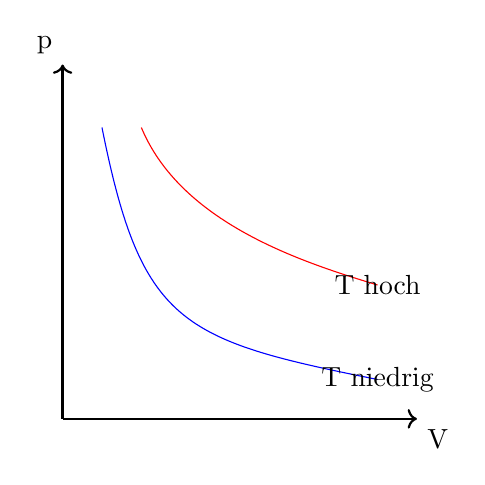
\begin{tikzpicture}
    \draw[thick,->] (0,0) -- (4.5,0) node[anchor=north west] {V};
    \draw[thick,->] (0,0) -- (0,4.5) node[anchor=south east] {p};
    \draw[blue] (0.5 ,3.7) .. controls (1 ,1.2) and (1.5 ,1) .. (4 ,0.5) node[] {\textcolor{black}{T niedrig}};
    \draw[red] (1 ,3.7) .. controls (1.5 ,2.5) and (3 ,2) .. (4 ,1.7) node[] {\textcolor{black}{T hoch}};
\end{tikzpicture}\\
\begin{equation*}
    p \alpha \frac{1}{V}
\end{equation*}\\
\begin{equation*}
    pV = \mathbf{konst}
\end{equation*}\\
isotherm\\\\
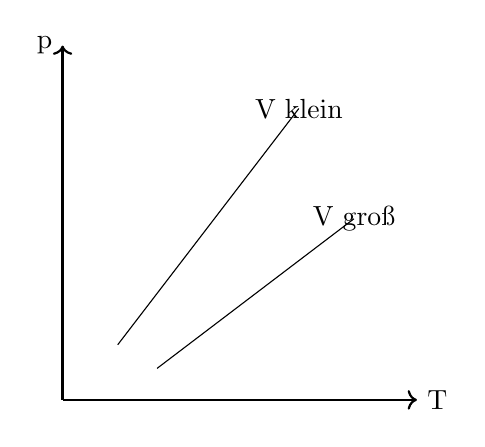
\begin{tikzpicture}
    \draw[thick,->] (0,0) -- (4.5,0) node[anchor=west] {T};
    \draw[thick,->] (0,0) -- (0,4.5) node[anchor=east] {p};
    \draw(0.7 ,0.7) -- (3, 3.7) node[] {V klein};
    \draw(1.2 ,0.4) -- (3.7, 2.3) node[] {V groß};
\end{tikzpicture}\\
\begin{equation*}
    p \alpha T
\end{equation*}
isochor\newpage
\begin{tikzpicture}
    \draw[thick,->] (0,0) -- (4.5,0) node[anchor=west] {V};
    \draw[thick,->] (0,0) -- (0,4.5) node[anchor=east] {T};
    \draw(0.7 ,0.7) -- (3, 3.7) node[] {p klein};
    \draw(1.2 ,0.4) -- (3.7, 2.3) node[] {p groß};
\end{tikzpicture}\\
\begin{equation*}
    V \alpha T
\end{equation*}
isobar\\\\
\subsubsection{ideale Gasgleichung $pV = nRT$ bzw. $pV_m = RT$}
$R = 8.314 \frac{\mathrm{J}}{\mathrm{K} \cdot \mathrm{mol}}$ allgemeine Gaskonstante\\
\begin{equation*}
    R = k N_A
\end{equation*}
wobei k die Boltzmannkonstante ist\\\\
$p^o = 1 \mathrm{bar}$\\\\
SATP:
\begin{itemize}
    \item $T=298.15$ K
    \item $p = p^o$
    \item $V_m = 24.789 \frac{\mathrm{dm^3}}{ mol}$
\end{itemize}
STP:
\begin{itemize}
    \item $T=273.15$ K = $0$ °C
    \item $p = p^o$
    \item $V_m = 22.414 \frac{\mathrm{dm^3}}{ mol}$
\end{itemize}
\begin{equation*}
    V(T,p,n) => dV=\left(\frac{\partial V}{\partial T}\right)dT+\left(\frac{\partial V}{\partial p}\right)dp+\left(\frac{\partial V}{\partial n}\right)dn
\end{equation*}
die partiellen Ableitungen sind:\\
thermische Ausdehnung, Komprassibilität, molares Volumen\\
\subsection{kinetische Gastheorie}
\begin{tikzpicture}
    \pgfmathsetmacro{\cubex}{7}
    \pgfmathsetmacro{\cubey}{4}
    \pgfmathsetmacro{\cubez}{4}
    \draw (0,0,0) -- ++(-\cubex,0,0) -- ++(0,-\cubey,0) -- ++(\cubex,0,0) -- cycle;
    \draw (0,0,0) -- ++(0,0,-\cubez) -- ++(0,-\cubey,0) -- ++(0,0,\cubez) -- cycle;
    \draw (0,0,0) -- ++(-\cubex,0,0) -- ++(0,0,-\cubez) -- ++(\cubex,0,0) -- cycle;
    \end{tikzpicture}\\
in diesem Raum bewegen sich kleine Gasteilchen.
\begin{itemize}
    \item Mittlere Geschwindigkeit $<v>$
    \item Stöße elastisch
\end{itemize}
Parameter:
\begin{itemize}
    \item Fläche $A$
    \item Volumen $V$
    \item Teilchenanzahl $N$
\end{itemize}
Zahl der Stöße in einer kleinen Zeit $dt$:
\begin{equation*}
    \frac{1}{6} \frac{N}{V}A\langle v\rangle dt
\end{equation*}
Impulsübertragung:
\begin{equation*}
    2m\langle v \rangle
\end{equation*}
Übertragender Impuls:
\begin{equation*}
    dp_A = \frac{1}{3}\frac{N}{V}Am \langle v \rangle ^2 dt
\end{equation*}
Wichtig: $p_A$ ist hier der Impuls
\begin{equation*}
    \frac{dp_A}{dt}=\frac{d\left(mv\right)}{dt}=m\frac{dv}{dt}=ma=F; p = \frac{F}{A}=\frac{1}{3}\frac{N}{V}m\langle v\rangle ^2= \frac{1}{3}\frac{N}{V}m \langle v^2 \rangle
\end{equation*}
Wichtig: $p$ ist hier wieder der Druck
\end{document}